\documentclass[12pt,a4paper]{article}

\usepackage[utf8]{inputenc}
\usepackage[T1]{fontenc}
\usepackage[brazil]{babel}
\usepackage[margin=2.5cm]{geometry}
\usepackage{graphicx}
\graphicspath{{relatorio/arquivos_auxiliares/}{../arquivos_auxiliares/}}
\usepackage{float}
\usepackage{amsmath}
\usepackage{amssymb}
\usepackage{booktabs}
\usepackage{array}
\usepackage{longtable}
\usepackage{listings}
\usepackage{xcolor}
\usepackage{setspace}
\usepackage{hyperref}
\hypersetup{colorlinks=true, linkcolor=black, urlcolor=blue}

% Placeholder para figuras ainda não inseridas
\newcommand{\figplaceholder}[1]{%
  \begin{figure}[H]
    \centering
    \fbox{\parbox{0.85\linewidth}{\centering\vspace{1.5cm}\textit{#1}\vspace{1.5cm}}}
    \caption{#1}
  \end{figure}}

% Estilo para trechos de código / nomes de arquivo
\lstset{basicstyle=\ttfamily\small, breaklines=true}

\onehalfspacing

\begin{document}

% capa
\begin{titlepage}
  \centering
  \vspace*{1cm}

  {\large Universidade de Brasília (UnB)\par}
  {\large Disciplina: Teleinformática e Redes 1 (TR1)\par}
  {\large Professor: Marcelo Antonio Marotta\par}

  \vspace{3cm}

  {\Huge\bfseries Simulador TR1\par}
  \vspace{0.4cm}
  {\LARGE\bfseries Camadas Física e de Enlace\par}
  \vspace{0.6cm}
  {\Large Trabalho Final\par}

  \vspace{2cm}

  
\includegraphics[width=0.4\linewidth]{logo_unb.png}

  \vspace{2cm}

  {\large\bfseries Integrantes do Grupo:\par}
  \vspace{0.3cm}
  {\large Gustavo Henrique Andrade Cavalcanti\par}
  {\large Fernando Augusto Hortencio\par}

  \vfill
  {\large Brasília --- 2026\par}
\end{titlepage}

% introducao
\section{Introdução}

O \textbf{Simulador TR1} simula a transmissao de uma mensagem de texto entre dois nos de uma rede, de forma didatica e fiel. Ele foi desenvolvido na disciplina de Teleinformatica e Redes 1 (TR1).

O foco e exercitar, de ponta a ponta, as camadas fisica e de enlace do modelo de protocolos. Isso abrange o enquadramento dos dados, a deteccao e a correcao de erros, a modulacao em banda-base e a modulacao por portadora. A mensagem atravessa um meio de comunicacao ruidoso, modelado por amostras em Volts somadas a ruido gaussiano.

Para o usuario, o uso e direto. Ele digita um texto e escolhe, na interface grafica, os protocolos de cada camada e os parametros de ruido do canal.

A partir dessas escolhas, o simulador converte o texto em bits (camada de aplicacao), monta os quadros com os codigos de deteccao, o Hamming e o enquadramento (camada de enlace) e transforma os bits em sinal eletrico, com modulacao banda-base ou por portadora (camada fisica). O sinal propaga pelo meio, que soma ruido gaussiano, e percorre o caminho inverso no receptor.

O resultado aparece em paginas simples de navegacao: Processamento, Bits e quadros, e Graficos. Elas mostram os bits de cada etapa, o texto recuperado, o relatorio de quadros e metricas como potencias, relacao sinal-ruido (SNR) e contagem de erros.

Um diferencial exigido pelo enunciado e a separacao explicita entre transmissor e receptor. Os dois executam em \textit{threads} independentes, que se comunicam apenas por filas (\texttt{queue.Queue}). As filas fazem o papel do meio fisico.

O ruido e somado justamente no canal, entre as duas \textit{threads}. Assim, o meio fica como o unico ponto de contato entre transmissor e receptor.

% arquitetura
\section{Arquitetura do Simulador}

O simulador foi escrito em Python 3. A interface grafica usa PyGObject (GTK 3), e os graficos dos sinais sao desenhados no proprio GTK com \texttt{Gtk.DrawingArea}. Assim, os protocolos e a visualizacao principal nao dependem de bibliotecas externas de calculo ou plotagem.

O enunciado exige os modulos \texttt{CamadaFisica}, \texttt{CamadaEnlace}, \texttt{InterfaceGUI} e \texttt{Simulador}. O projeto entrega esses modulos em \textit{snake\_case} (padrao da linguagem) e acrescenta modulos auxiliares para a camada de aplicacao, o meio de comunicacao e a suite de testes.

A Tabela~\ref{tab:arquivos} resume o papel de cada arquivo e o requisito que ele atende.

\begin{table}[H]
  \centering
  \small
  \caption{Mapeamento de arquivos do projeto e requisitos do enunciado.}
  \label{tab:arquivos}
  \begin{tabular}{>{\ttfamily}p{3.8cm} p{7.0cm} p{2.2cm}}
    \toprule
    \normalfont\textbf{Arquivo} & \textbf{Papel} & \textbf{Requisito} \\
    \midrule
    simulador.py & Rotina principal: orquestra TX $\rightarrow$ meio $\rightarrow$ RX em \textit{threads} & Simulador \\
    camada\_fisica.py & Modulação digital (banda-base) e por portadora & CamadaFisica \\
    camada\_enlace.py & Enquadramento, detecção e correção de erros & CamadaEnlace \\
    interface\_gui.py & GUI em GTK 3 (entrada, configuração, gráficos) & InterfaceGUI \\
    camada\_aplicacao.py & Texto $\leftrightarrow$ bits (codificador/decodificador) & apoio \\
    meio\_comunicacao.py & Canal: sinal em Volts + ruído gaussiano $n(x,\sigma)$ & apoio (meio) \\
    testes.py & Suíte de testes de ida-e-volta (TX$\rightarrow$RX sem ruído == entrada) & validação \\
    \bottomrule
  \end{tabular}
\end{table}

\subsection{Diagrama de Pilha \texorpdfstring{(TX $\rightarrow$ MEIO $\rightarrow$ RX)}{(TX -> MEIO -> RX)}}

No transmissor, o texto desce pelas camadas de aplicacao, enlace e fisica ate virar um sinal eletrico. No meio, o ruido gaussiano e somado amostra a amostra. No receptor, o sinal sobe de volta pelas camadas ate ser reconstruido como texto. A comunicacao entre as \textit{threads} ocorre por duas filas: TX $\to$ [canal soma ruído] $\to$ RX.

\begin{figure}[H]
  \centering
  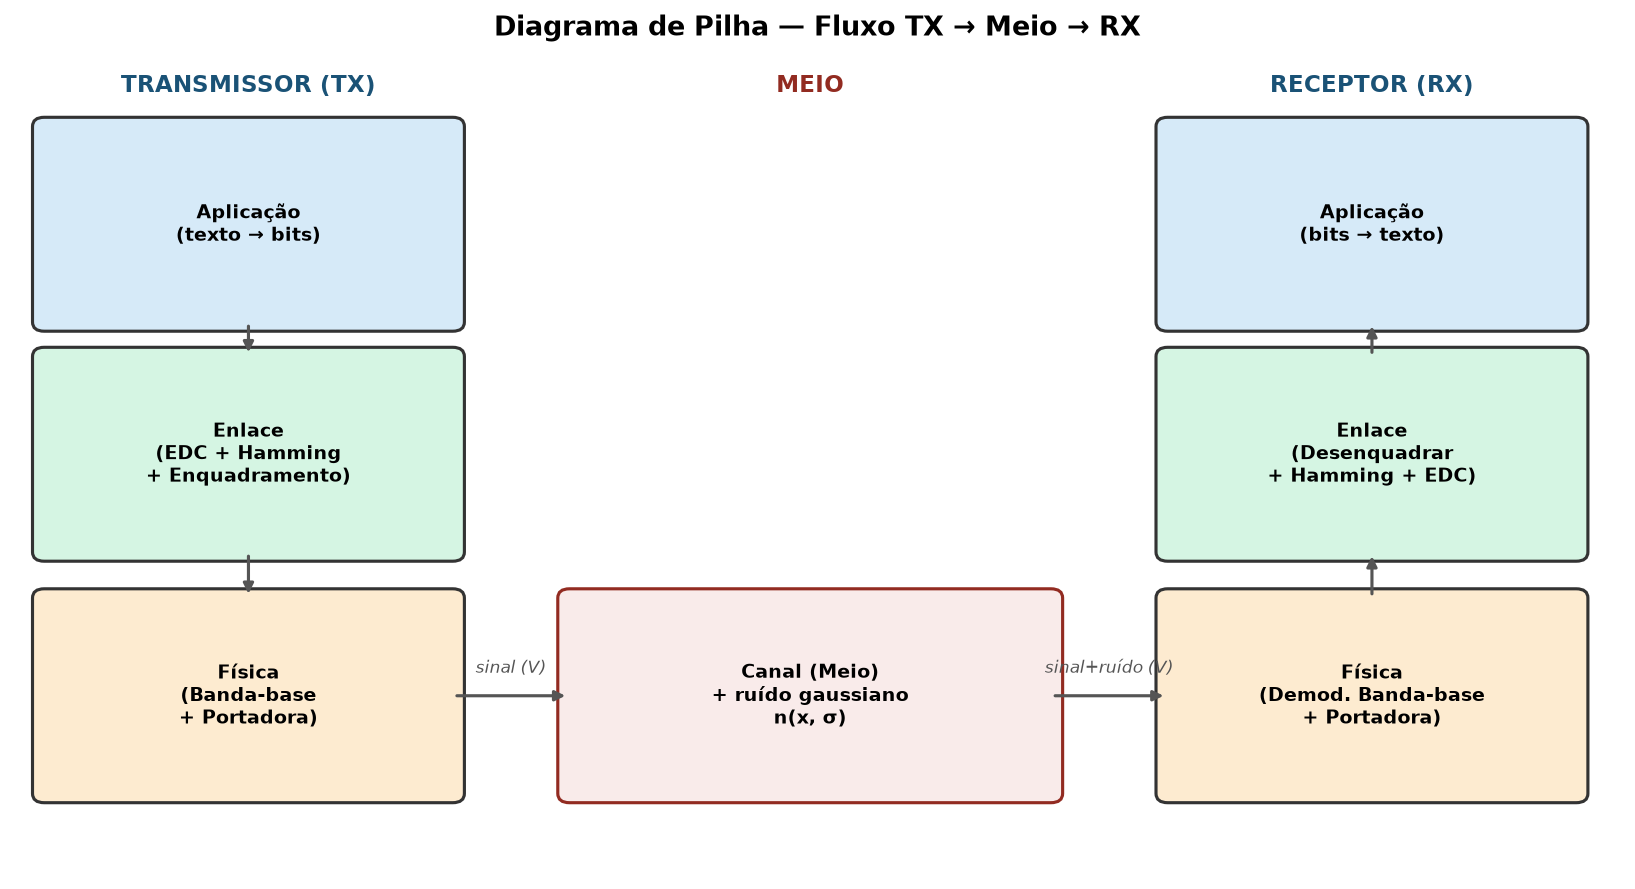
\includegraphics[width=0.92\linewidth]{diagrama_pilha.png}
  \caption{Diagrama de pilha TX $\to$ Meio $\to$ RX, com as camadas Aplicação, Enlace e Física no transmissor e no receptor e o canal somando ruído gaussiano.}
  \label{fig:diagrama_pilha}
\end{figure}

% implementacao
\section{Implementação}

Esta secao detalha cada camada: o funcionamento dos protocolos e as decisoes de projeto.

Os algoritmos centrais (CRC, Hamming, checksum e todas as modulacoes) foram implementados manualmente, bit a bit, sem bibliotecas externas como a \texttt{zlib}, conforme exige o enunciado.

Os parametros globais da camada fisica sao: $V = 1{,}0$~V de amplitude, 100 amostras por bit, 100 amostras por simbolo, 4 ciclos de portadora por simbolo e o par de frequencias $(2,4)$ ciclos para o FSK.

\subsection{Camada Física --- Modulação Digital (Banda-Base)}

Foram implementadas tres codificacoes de linha.

No \textbf{NRZ-Polar}, o bit 1 vira $+V$ e o bit 0 vira $-V$. No receptor, a decisao usa a media das amostras de cada bit.

No \textbf{Manchester}, adota-se a convencao de Tanenbaum/G.E.~Thomas: XOR com o clock. O bit 0 e uma transicao de baixo para alto e o bit 1, de alto para baixo. A decisao compara a media da primeira metade do periodo com a da segunda.

No \textbf{Bipolar (AMI)}, o bit 0 corresponde a 0~V e o bit 1 alterna entre $+V$ e $-V$, o que elimina a componente DC. A decisao usa o criterio $|\text{media}| > V/2$.

As funcoes seguem o padrao \texttt{modular\_x} / \texttt{demodular\_x} para cada esquema.

\begin{figure}[H]
  \centering
  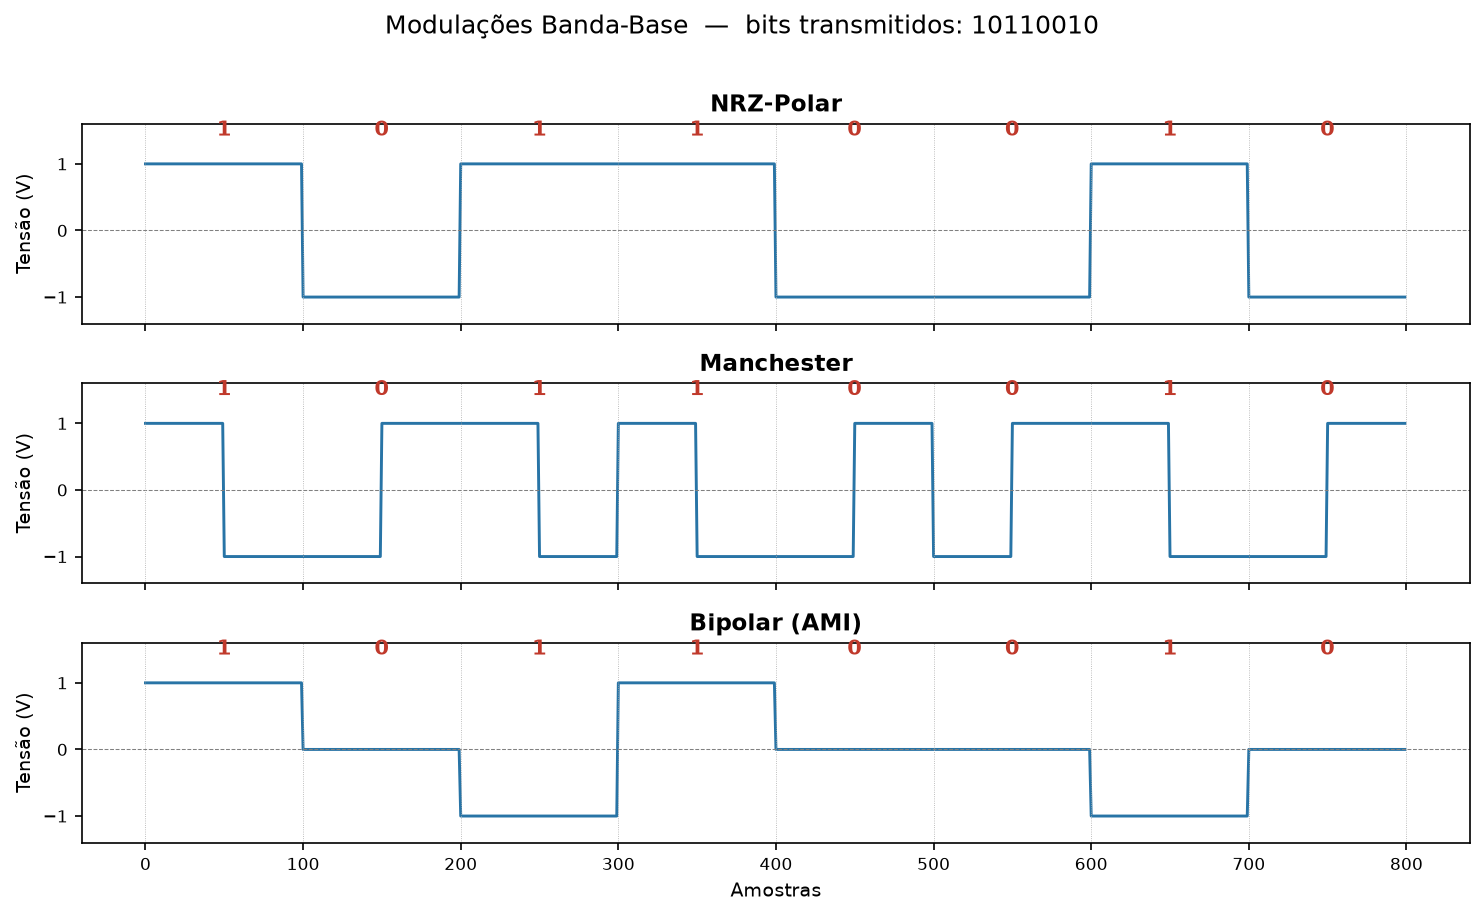
\includegraphics[width=0.92\linewidth]{sinais_banda_base.png}
  \caption{Formas de onda das modulações banda-base (NRZ-Polar, Manchester e Bipolar) para a sequência de bits \texttt{10110010}.}
  \label{fig:sinais_banda_base}
\end{figure}

\subsection{Camada Física --- Modulação por Portadora}

As modulacoes por portadora usam uma representacao comum em I/Q, na forma $s(t) = I\cos(2\pi f t) - Q\operatorname{sen}(2\pi f t)$. A demodulacao e coerente, por correlacao (produto interno), e escolhe o ponto da constelacao mais proximo.

No \textbf{ASK} (on-off keying), o bit 1 e transmitido com a portadora em amplitude $V$ e o bit 0 com $0~V$; a decisao compara a amplitude medida com $V/2$.

No \textbf{FSK}, usam-se duas frequencias ortogonais (2 e 4 ciclos por simbolo) e a decisao olha em qual frequencia ha mais energia.

O \textbf{QPSK} transporta 2 bits por simbolo com mapeamento Gray. O \textbf{16-QAM} transporta 4 bits por simbolo, com niveis Gray $\{-3,-1,+1,+3\}\cdot(V/3)$ em cada eixo I e Q, decididos de forma independente.

Funcoes auxiliares como \texttt{onda}, \texttt{correlacionar}, \texttt{pad} e \texttt{bits\_do\_ponto\_mais\_proximo} sao reaproveitadas entre os esquemas.

\begin{figure}[H]
  \centering
  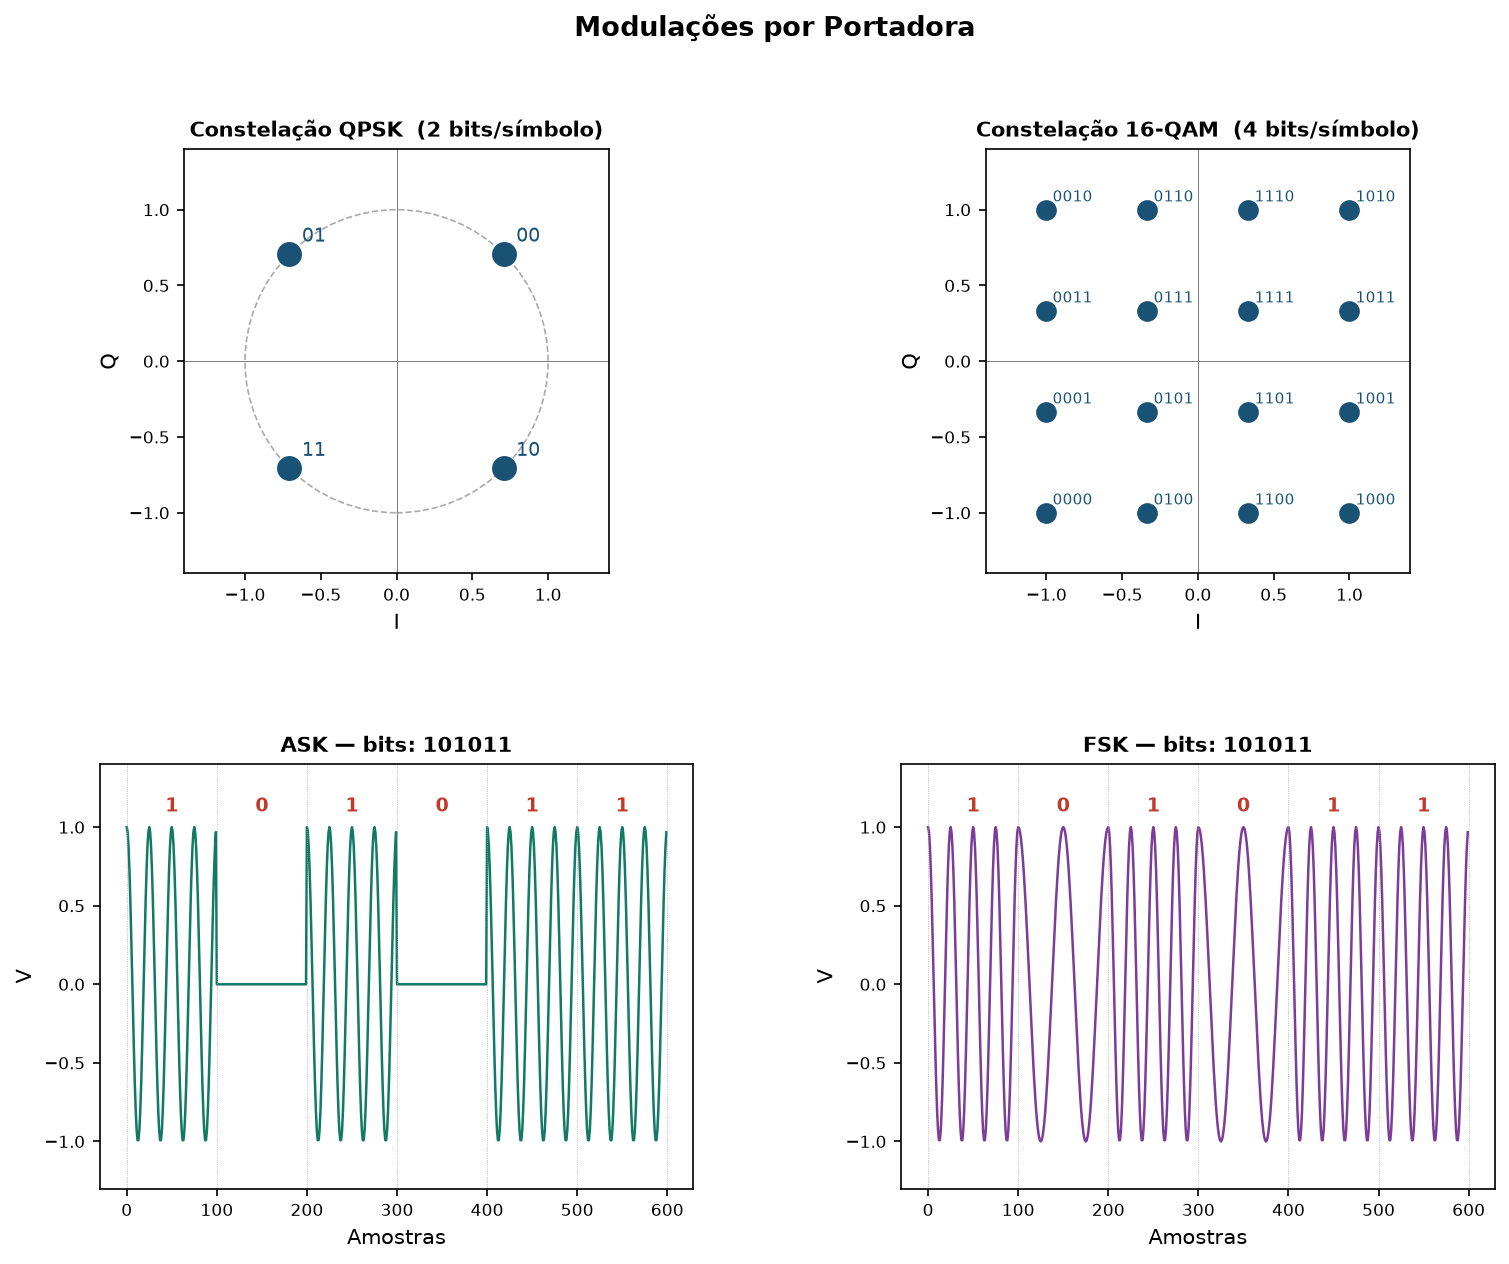
\includegraphics[width=0.95\linewidth]{constelacoes_portadora.png}
  \caption{Constelações QPSK (2~bits/símbolo) e 16-QAM (4~bits/símbolo) com mapeamento Gray, e formas de onda ASK e FSK para a sequência \texttt{101011}.}
  \label{fig:constelacoes}
\end{figure}

A Figura~\ref{fig:dispersao_ruido} ilustra como o ruído desloca os pontos da constelação QPSK, tornando a decisão de mínima distância progressivamente mais suscetível a erros.

\begin{figure}[H]
  \centering
  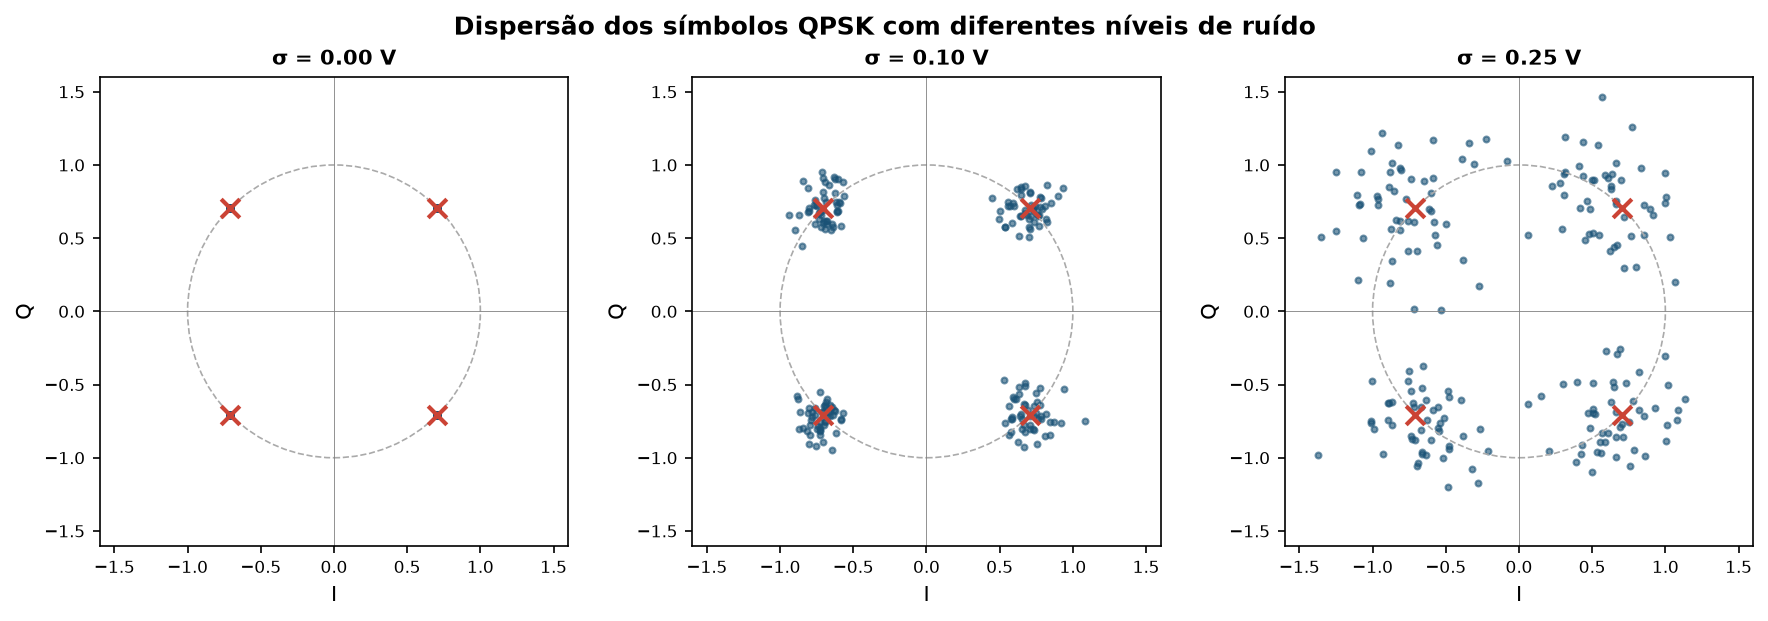
\includegraphics[width=0.95\linewidth]{qpsk_dispersao_ruido.png}
  \caption{Dispersão dos símbolos QPSK recebidos para três níveis de ruído ($\sigma = 0{,}00$, $0{,}10$ e $0{,}25$~V). A cruz vermelha marca o ponto ideal da constelação; os pontos azuis são os símbolos recebidos após o canal ruidoso.}
  \label{fig:dispersao_ruido}
\end{figure}

\subsection{Camada de Enlace --- Enquadramento}

Foram implementadas tres tecnicas de enquadramento.

Na \textbf{contagem de caracteres}, um byte de cabecalho indica o numero de bytes do payload, limitado a no maximo 255.

No \textbf{byte stuffing} (FLAGs com insercao de bytes), adota-se FLAG $=$ \texttt{0x7E} e ESC $=$ \texttt{0x7D}. Quando esses padroes aparecem nos dados, um byte ESC e inserido antes deles.

No \textbf{bit stuffing}, a FLAG e \texttt{01111110}. Apos cinco bits 1 consecutivos no payload, insere-se um bit 0 para garantir que a FLAG nunca apareca nos dados.

As funcoes seguem o padrao \texttt{enquadrar\_x} / \texttt{desenquadrar\_x}.

\subsection{Camada de Enlace --- Detecção de Erros}

Foram desenvolvidos tres mecanismos de deteccao de erros, todos sem bibliotecas externas.

O \textbf{bit de paridade par} anexa um byte (sete zeros mais o bit de paridade) para manter o alinhamento em bytes, e detecta um numero impar de bits invertidos.

O \textbf{checksum} usa a soma em complemento de 1 de palavras de 16 bits, com \textit{end-around carry}, exatamente como o checksum da Internet.

O \textbf{CRC-32} (IEEE 802) usa o polinomio 0x04C11DB7 na forma refletida 0xEDB88320, com inicializacao 0xFFFFFFFF e XOR final. Sua corretude foi validada contra o vetor de teste conhecido: \texttt{CRC32}("123456789") = 0xCBF43926.

As funcoes seguem o padrao \texttt{adicionar\_x} / \texttt{verificar\_x}.

\subsection{Camada de Enlace --- Correção de Erros (Hamming)}

A correcao de erros usa o codigo de \textbf{Hamming(8,4) estendido (SECDED)}, que transforma cada bloco de 4 bits em 8 bits. Ele corrige um erro e detecta dois erros por bloco.

A decodificacao combina a sindrome com o bit de paridade geral $p_0$. Se a sindrome e nao nula e a paridade acusa erro, ha um erro unico corrigivel. Se a sindrome e nao nula mas a paridade esta correta, detecta-se um erro duplo, que nao da para corrigir.

A escolha do Hamming estendido, em vez do (7,4) puro, foi deliberada: alem de detectar o erro duplo, ele mantem o alinhamento em bytes, ao dobrar 1 byte em 2 bytes.

\begin{figure}[H]
  \centering
  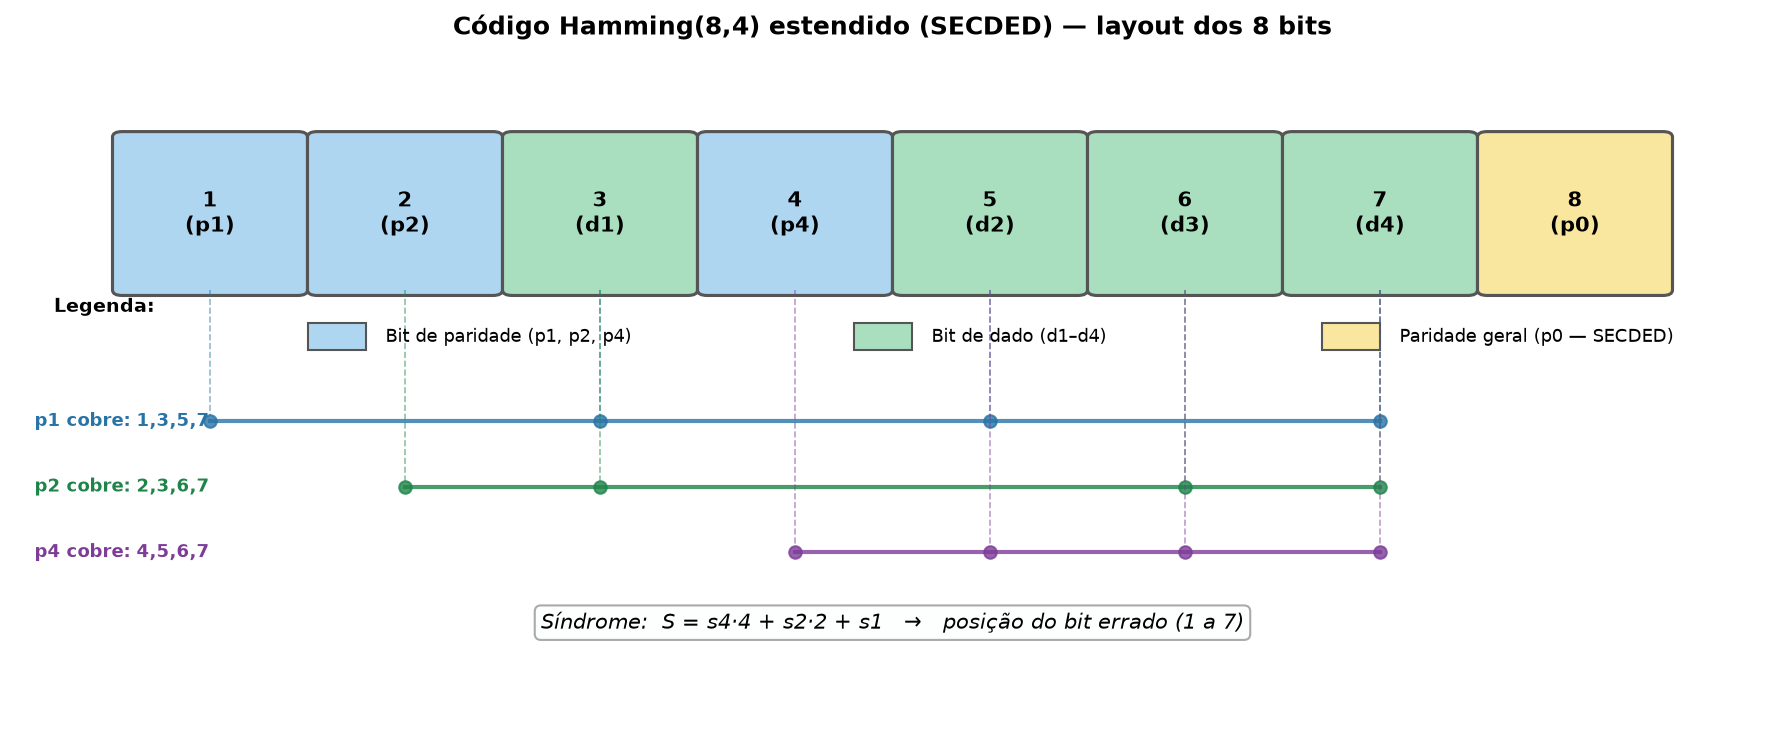
\includegraphics[width=0.95\linewidth]{hamming_8_4.png}
  \caption{Layout do bloco Hamming(8,4) estendido: posições dos bits de paridade ($p_1$, $p_2$, $p_4$, $p_0$) e de dado ($d_1$--$d_4$), coberturas de cada bit de paridade e fórmula da síndrome.}
  \label{fig:hamming}
\end{figure}

\subsection{Interface Gráfica (GTK 3)}

A interface foi feita em GTK 3 (nao em terminal), conforme exigido, pela classe \texttt{JanelaSimulador} em \texttt{interface\_gui.py}.

O painel esquerdo reune a configuracao: o texto de entrada, o tamanho maximo de quadro, os menus de enquadramento, deteccao, correcao, modulacao digital e modulacao por portadora, e os parametros de ruido $x$ e $\sigma$.

O painel direito mostra metricas gerais e tres paginas: Processamento, Bits e quadros, e Graficos. A pagina de processamento mostra a tabela fase a fase. A pagina de bits mostra os fluxos TX/RX, o relatorio por quadro (EDC OK ou com erro, bits corrigidos e erro duplo) e a marcacao simples dos bits: \texttt{p} para carga original e \texttt{+} para bits adicionados pelo protocolo. A pagina de graficos mostra quatro sinais desenhados diretamente em GTK: banda-base TX, sinal enviado ao meio, sinal recebido com ruido e banda-base reconstruida no RX. A separacao entre TX e RX fica explicita, atendendo ao enunciado.

\begin{figure}[H]
  \centering
  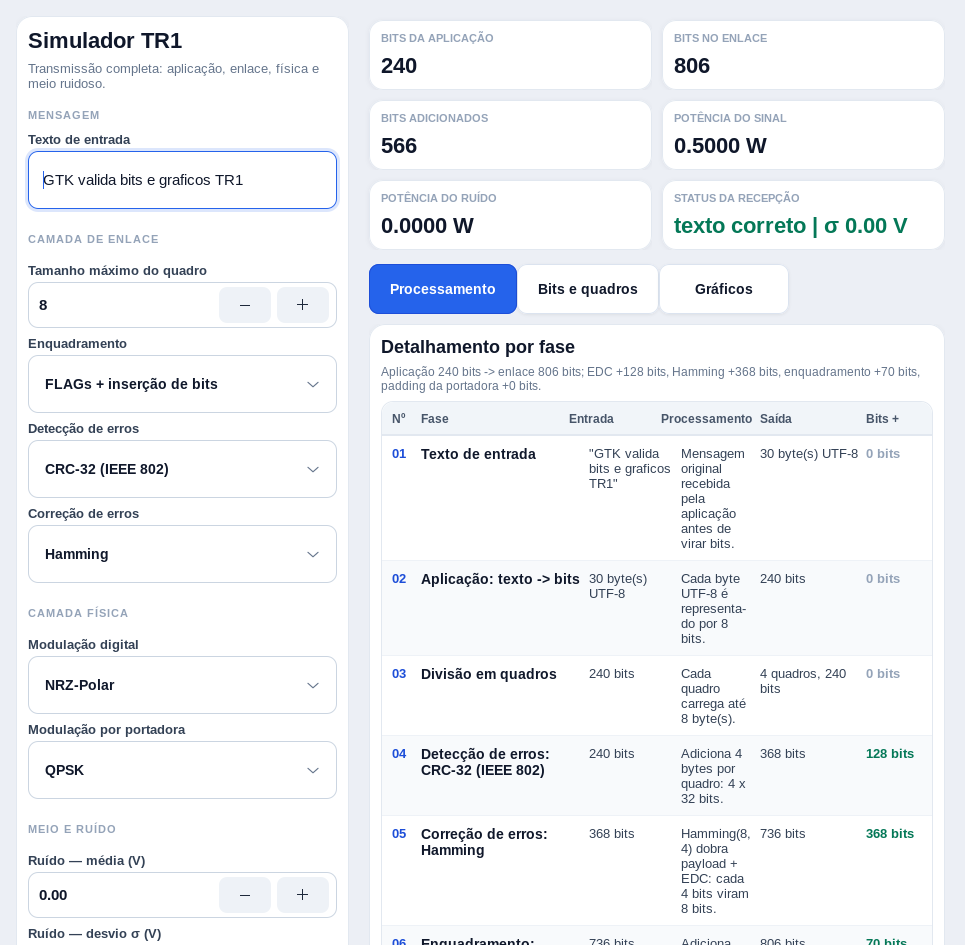
\includegraphics[width=0.92\linewidth]{interface_gtk.png}
  \caption{Interface gráfica em GTK 3: painel de configuração à esquerda, métricas no painel principal e páginas simples para processamento, bits/quadros e gráficos nativos dos sinais.}
  \label{fig:interface_gtk}
\end{figure}

\subsection{Fluxo dos Pipelines de Transmissão e Recepção}

No transmissor, \texttt{camada\_enlace.transmitir(bits, config)} divide os bits em blocos de ate \texttt{tam\_max\_quadro} bytes. A cada bloco anexa o codigo de deteccao (paridade, checksum ou CRC); se o Hamming estiver ativo, o conjunto payload mais EDC e codificado, dobrando de tamanho; e o bloco e enquadrado. Os quadros sao concatenados num unico fluxo de bits. Em seguida, \texttt{simulador.\_rotina\_tx} aplica a modulacao digital banda-base e, se houver portadora, a modulacao por portadora, gerando o sinal enviado ao meio.

No receptor, \texttt{simulador.\_rotina\_rx} recebe o sinal ruidoso e demodula a portadora (ou a banda-base). Entao \texttt{camada\_enlace.receber} desenquadra, corrige com Hamming, verifica o EDC e entrega os bits a \texttt{camada\_aplicacao.bits\_para\_texto}.

O meio, em \texttt{meio\_comunicacao.transmitir(sinal, media, sigma)}, soma \texttt{random.gauss(media, sigma)} a cada amostra (ruido AWGN). Quando \texttt{media} e $\sigma$ sao zero, ele se comporta como canal ideal. A funcao \texttt{potencia\_media} calcula $P$ como a media de $v^2$ (em watts sobre 1~$\Omega$), usada no calculo da SNR.

\begin{figure}[H]
  \centering
  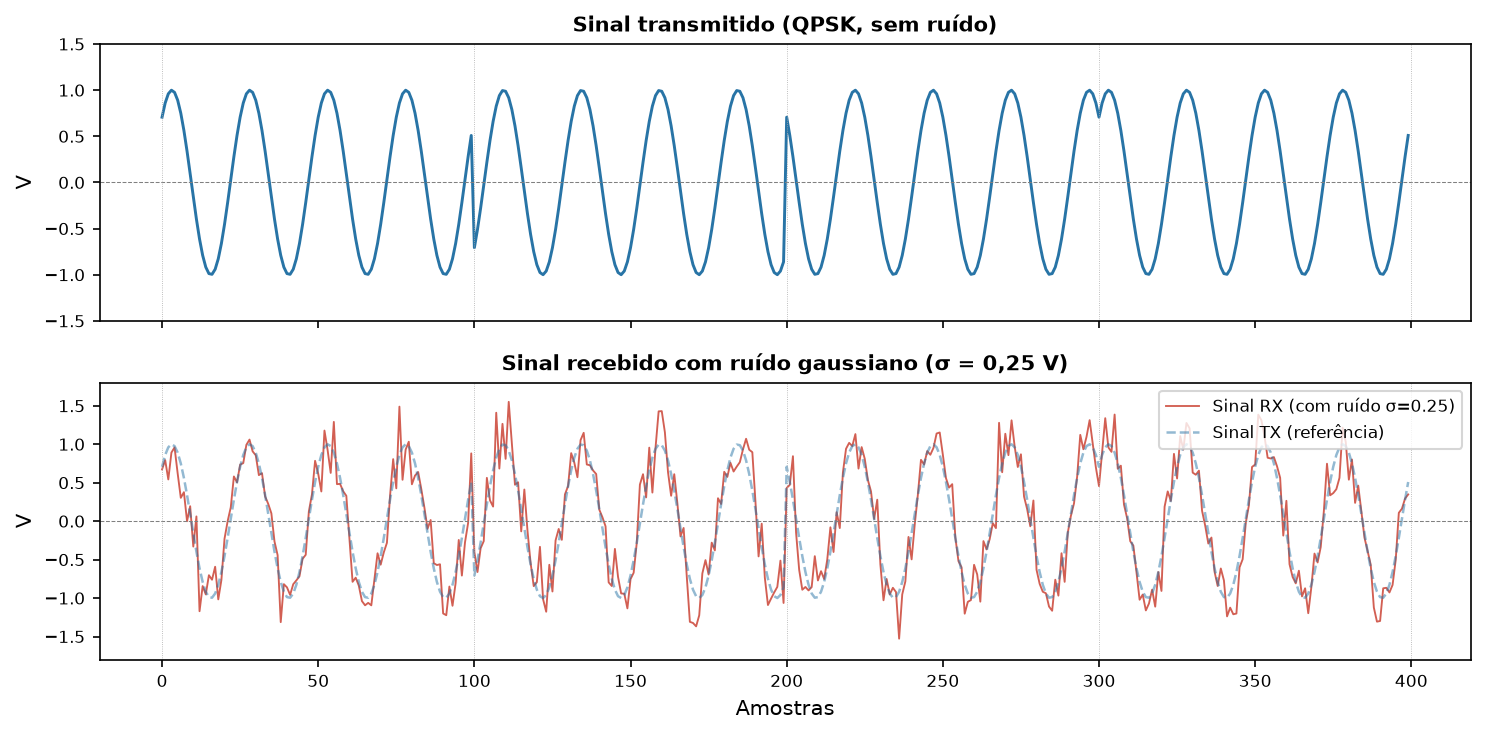
\includegraphics[width=0.92\linewidth]{sinal_com_ruido.png}
  \caption{Sinal QPSK transmitido (limpo) e sinal recebido com ruído gaussiano ($\sigma = 0{,}25$~V). A linha tracejada é o sinal original de referência.}
  \label{fig:sinal_ruido}
\end{figure}

\subsection{Decisões de Projeto e Casos Omissos}

Alguns pontos nao foram especificados no enunciado e exigiram decisoes de projeto.

Todos os EDCs foram alinhados em bytes (paridade 1 byte, checksum 2 bytes e CRC 4 bytes), para combinar com os enquadramentos, que operam sobre bytes.

A ordem de aplicacao e EDC primeiro e Hamming depois, para que o Hamming proteja tambem os bits de deteccao. No receptor, a ordem se inverte: corrige antes de verificar o EDC.

No QPSK e no 16-QAM, o sinal e completado com zeros ate fechar um simbolo inteiro (padding), e o desenquadramento descarta o excedente.

A convencao Manchester e a de Tanenbaum/G.E.~Thomas, documentada de forma explicita. A demodulacao foi feita robusta a ruido: por media na banda-base e por correlacao coerente com minima distancia na constelacao por portadora, aproveitando o mapeamento Gray para reduzir bits errados.

A contagem de caracteres e limitada a 255 bytes por quadro, validada em \texttt{transmitir()} com um \texttt{ValueError} exibido na GUI. A decodificacao de texto usa \texttt{errors="replace"}, para nao interromper o programa quando o ruido corrompe bytes.

Por fim, o GTK e importado apenas no contexto da GUI, o que permite rodar os testes e os modulos em maquinas sem GTK.

% validacao
\section{Validação e Resultados}

A corretude do simulador e verificada pela suite \texttt{testes.py}, com o criterio de ida-e-volta: sem ruido, a saida do receptor deve ser identica a entrada do transmissor.

Os testes cobrem: a camada de aplicacao (texto para bits e de volta, incluindo acentos UTF-8); os tres enquadramentos, com seus casos criticos (payload so de bits 1 no bit stuffing e ocorrencia de FLAG/ESC no byte stuffing); os tres EDCs (aceitando quadros integros e detectando um bit invertido), com a conferencia do CRC-32 contra 0xCBF43926; o Hamming (ida-e-volta, correcao de um bit e deteccao de erro duplo); todas as modulacoes banda-base e por portadora, com e sem ruido; e a simulacao completa, combinando os 3 enquadramentos com as 5 opcoes de portadora.

O resultado atual da execucao e ``TODOS OS TESTES PASSARAM'', o que evidencia a corretude da implementacao.

\begin{figure}[H]
  \centering
  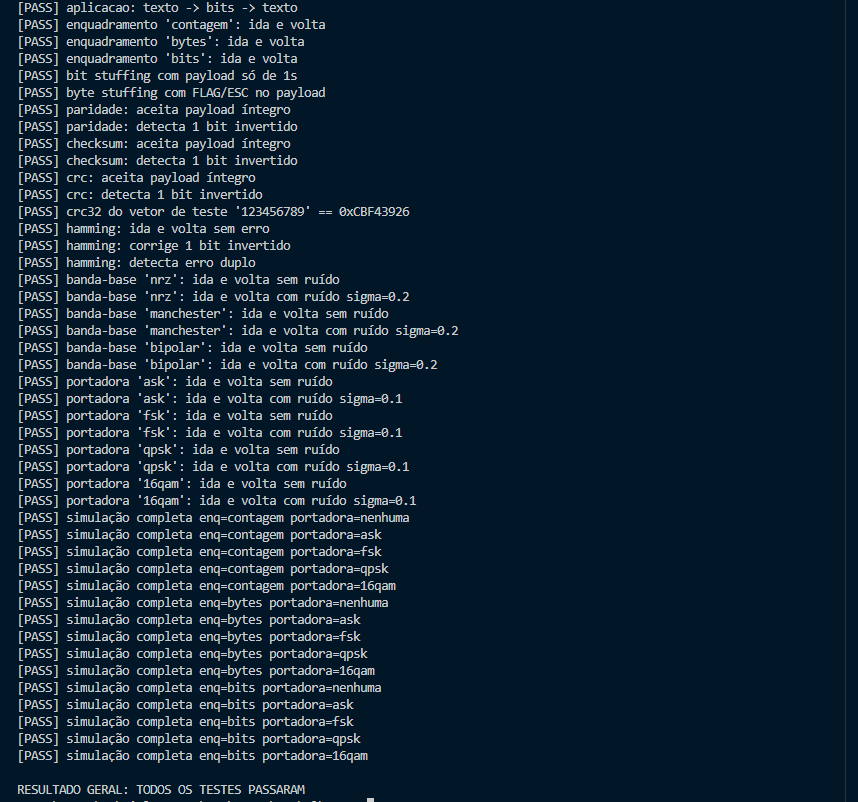
\includegraphics[width=0.85\linewidth]{testes_terminal.png}
  \caption{Saída do terminal após execução de \texttt{testes.py}: todos os 45 testes passaram.}
  \label{fig:testes_terminal}
\end{figure}

% membros
\section{Membros e Atividades Desenvolvidas}

O trabalho foi dividido entre os dois integrantes do grupo, mantendo uma separacao equilibrada entre protocolos, simulacao e interface.

\textbf{Gustavo Henrique Andrade Cavalcanti} ficou responsavel pela camada fisica e por parte da camada de enlace: modulacoes banda-base (NRZ-Polar, Manchester e Bipolar), modulacoes por portadora (ASK, FSK, QPSK e 16-QAM), meio de comunicacao com ruido gaussiano, enquadramento e mecanismos de deteccao e correcao de erros.

\textbf{Fernando Augusto Hortencio} ficou responsavel pela integracao do simulador, pela comunicacao entre as \textit{threads} de transmissor e receptor por filas, pela interface grafica em GTK, pela interface web opcional, pela organizacao do repositorio, pela documentacao e pela validacao final com testes de ida-e-volta.

Apesar dessa divisao, ambos revisaram os pontos centrais do projeto para dominar a explicacao completa do codigo durante a apresentacao.

% conclusao
\section{Conclusão}

O Simulador TR1 atingiu os objetivos propostos. Ele implementa todos os protocolos exigidos das camadas fisica e de enlace sem usar bibliotecas externas nos algoritmos centrais: CRC, Hamming, checksum e todas as modulacoes foram escritos manualmente, bit a bit.

A arquitetura baseada em \textit{threads} de transmissor e receptor reproduz fielmente o diagrama do enunciado e isola o meio, com o ruido gaussiano, como o unico ponto de contato entre as duas pontas.

As principais dificuldades foram: a demodulacao robusta a ruido, que exigiu correlacao coerente e criterio de minima distancia na constelacao; a manutencao do alinhamento em bytes entre EDC, Hamming e enquadramento; o tratamento do padding nas modulacoes multibit QPSK e 16-QAM; e a definicao e documentacao explicita da convencao de Manchester.

Superados esses pontos, a suite de testes de ida-e-volta passou em todos os casos, confirmando a corretude do sistema.

O resultado e uma ferramenta didatica que torna tangiveis os conceitos das camadas fisica e de enlace, permitindo observar, na pratica, o efeito do ruido, dos esquemas de modulacao e dos mecanismos de deteccao e correcao de erros sobre a transmissao de dados.

\end{document}
